\documentclass[a4paper,openright,10pt]{article}
\usepackage[spanish]{babel} 
\usepackage[utf8]{inputenc}
\usepackage[usenames]{color}
\usepackage[T1]{fontenc}
\usepackage{lmodern}
\usepackage{float}
%Formato figuras
\usepackage{graphicx}
\usepackage{minted}
%Márgenes
\usepackage[left=2.5cm,top=2.5cm,right=2.0cm,bottom=2.5cm]{geometry}
\usepackage[hidelinks]{hyperref} 
\usepackage[usenames]{color}

\graphicspath{{./Figuras/}}



\begin{document}


%PORTADA
\pagestyle{empty} %Quitar el formato predeterminado a la primera hoja
\begin{center}
\vspace*{-1.5cm}
\begin{figure}
\centering
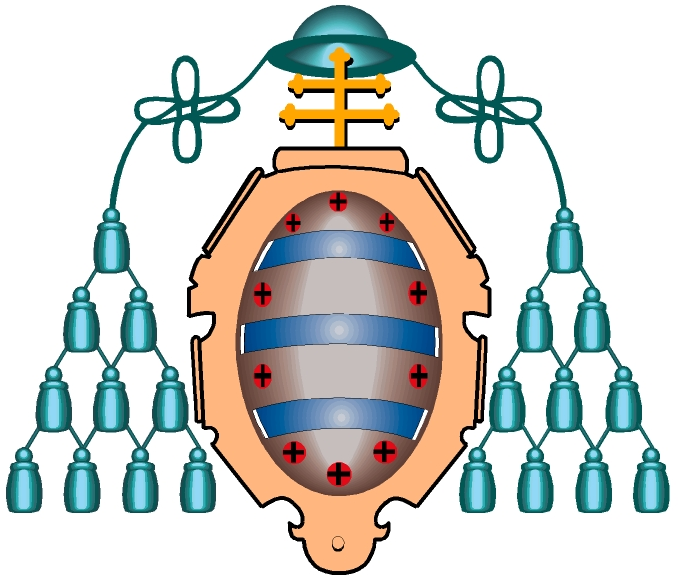
\includegraphics[width=4cm]{uniovi.png}
\end{figure}
\vspace*{0.5cm}
\rule{80mm}{0.1mm}

\begin{Large}

Universidad de Oviedo
	
\end{Large}

Escuela Politécnica de Ingeniería de Gijón

\vspace*{3cm}

\begin{Large}

Grado en Tecnologías y Servicios de la Telecomunicación
	
\end{Large}

\vspace*{0.17cm}

Prácticas externas

\vspace*{1cm}

\begin{huge}

Alechip Soluciones Informáticas S.L.

\end{huge}

\vspace*{0.5cm}

Marco Martínez Ávila
	
\end{center}

\begin{center}
	
\vspace*{2cm}
\centering

\includegraphics[width=3cm]{logo.png}
	
	
\end{center}

\clearpage

\pagestyle{plain} %Añadir numeración a las páginas siguientes


\section {Descripción de la práctica}

Esta práctica consiste en la elaboración de un cliente y servidor que se comuniquen utilizando el protocolo SNF, incluyendo esta vez números de secuencia.

\section{Descripción del trabajo realizado}

La parte de mayor importancia, más allá de programar el código, resultó ser la elaboración del diagrama SDL y de los distintos casos expuestos mediante MSC. Al fin y al cabo, no dejaba de ser planificar cómo íbamos a llevar cabo la implementación, por lo que no tener dudas al respecto fue imprescindible desde un primer momento. Una vez finalizada esta primera etapa, sólo fue necesario llevar al Visual Studio lo estipulado en el SDL; los MSC, por su parte, fueron importantes de cara a complementar al primero, ya que gracias a los distintos casos a tener en cuenta fue posible ir perfilando de la forma correcta el diagrama. Este aspecto ha resultado interesante, ya que en ninguna ocasión habíamos tenido que elaborar antes estos esquemas, descubriendo ahora lo útiles que resultan.

El formato de los mensajes es, posiblemente, otro punto destacable. En un principio se pensó juntar el número de secuencia y el de interés en uno sólo, utilizando la siguiente instrucción.

\begin{minted}{csharp}
	int newNumber = int.Parse(a.ToString() + b.ToString())
\end{minted}

Sin embargo, se decidió descartar esta opción, ya que concatenar números elevados limitaba muchísimo los valores que se podían enviar, al depender del rango disponible para el \textit{int} resultante; Por lo tanto, se tomó la decisión de usar un separador como el la práctica 1, de forma que en el receptor se trataran los dos números de forma independiente.

En lo que respecta a los problemas encontrados en la práctica anterior con la decodificación y los stream, no ha habido problemas esta vez. Esto es debido al uso del sockets UDP, que como se ha explicado en clase, posibilitan la transferencia de información mediante paquetes, en lugar de mediante un stream.

\section{Conclusiones}

La realización de la práctica 1, y todos las dificultades derivadas, resultaron de gran ayuda de cara a la resolución de esta. Por lo tanto, resultó mucho más sencillo concluir esta satisfactoriamente, aunque merece la pena destacar la importancia del SDL y de los MSC. Teniendo estos diagramas claros y realizados de forma correcta, escribir el código no deja de ser llevar los esquemas a texto de programación, lo que requiere mucho menos razonamiento que comenzar directamente con esta etapa.

\end{document}